% Options for packages loaded elsewhere
\PassOptionsToPackage{unicode}{hyperref}
\PassOptionsToPackage{hyphens}{url}
\documentclass[
  ignorenonframetext,
]{beamer}
\newif\ifbibliography
\usepackage{pgfpages}
\setbeamertemplate{caption}[numbered]
\setbeamertemplate{caption label separator}{: }
\setbeamercolor{caption name}{fg=normal text.fg}
\beamertemplatenavigationsymbolsempty
% remove section numbering
\setbeamertemplate{part page}{
  \centering
  \begin{beamercolorbox}[sep=16pt,center]{part title}
    \usebeamerfont{part title}\insertpart\par
  \end{beamercolorbox}
}
\setbeamertemplate{section page}{
  \centering
  \begin{beamercolorbox}[sep=12pt,center]{section title}
    \usebeamerfont{section title}\insertsection\par
  \end{beamercolorbox}
}
\setbeamertemplate{subsection page}{
  \centering
  \begin{beamercolorbox}[sep=8pt,center]{subsection title}
    \usebeamerfont{subsection title}\insertsubsection\par
  \end{beamercolorbox}
}
% Prevent slide breaks in the middle of a paragraph
\widowpenalties 1 10000
\raggedbottom
\AtBeginPart{
  \frame{\partpage}
}
\AtBeginSection{
  \ifbibliography
  \else
    \frame{\sectionpage}
  \fi
}
\AtBeginSubsection{
  \frame{\subsectionpage}
}
\usepackage{iftex}
\ifPDFTeX
  \usepackage[T1]{fontenc}
  \usepackage[utf8]{inputenc}
  \usepackage{textcomp} % provide euro and other symbols
\else % if luatex or xetex
  \usepackage{unicode-math} % this also loads fontspec
  \defaultfontfeatures{Scale=MatchLowercase}
  \defaultfontfeatures[\rmfamily]{Ligatures=TeX,Scale=1}
\fi
\usepackage{lmodern}
\ifPDFTeX\else
  % xetex/luatex font selection
\fi
% Use upquote if available, for straight quotes in verbatim environments
\IfFileExists{upquote.sty}{\usepackage{upquote}}{}
\IfFileExists{microtype.sty}{% use microtype if available
  \usepackage[]{microtype}
  \UseMicrotypeSet[protrusion]{basicmath} % disable protrusion for tt fonts
}{}
\makeatletter
\@ifundefined{KOMAClassName}{% if non-KOMA class
  \IfFileExists{parskip.sty}{%
    \usepackage{parskip}
  }{% else
    \setlength{\parindent}{0pt}
    \setlength{\parskip}{6pt plus 2pt minus 1pt}}
}{% if KOMA class
  \KOMAoptions{parskip=half}}
\makeatother
\usepackage{graphicx}
\makeatletter
\newsavebox\pandoc@box
\newcommand*\pandocbounded[1]{% scales image to fit in text height/width
  \sbox\pandoc@box{#1}%
  \Gscale@div\@tempa{\textheight}{\dimexpr\ht\pandoc@box+\dp\pandoc@box\relax}%
  \Gscale@div\@tempb{\linewidth}{\wd\pandoc@box}%
  \ifdim\@tempb\p@<\@tempa\p@\let\@tempa\@tempb\fi% select the smaller of both
  \ifdim\@tempa\p@<\p@\scalebox{\@tempa}{\usebox\pandoc@box}%
  \else\usebox{\pandoc@box}%
  \fi%
}
% Set default figure placement to htbp
\def\fps@figure{htbp}
\makeatother
\setlength{\emergencystretch}{3em} % prevent overfull lines
\providecommand{\tightlist}{%
  \setlength{\itemsep}{0pt}\setlength{\parskip}{0pt}}
\usepackage{bookmark}
\IfFileExists{xurl.sty}{\usepackage{xurl}}{} % add URL line breaks if available
\urlstyle{same}
\hypersetup{
  pdftitle={Introduction},
  hidelinks,
  pdfcreator={LaTeX via pandoc}}

\title{\texorpdfstring{Introduction}{Introduction}}
\author{\texorpdfstring{}{}}
\date{}

\begin{document}
\frame{\titlepage}

\section{Introduction}\label{sec:introduction}

\begin{frame}{The Problem of Case Assignment in Cognitive Scenarios}
\protect\phantomsection\label{the-problem-of-case-assignment-in-cognitive-scenarios}
Every natural language encodes relational structure---\emph{who does
what to whom, with what, where, and why}---through some form of case
system. In morphologically rich languages such as Finnish, Latin, or
Sanskrit, this encoding is overt: distinct suffixes mark the agent,
patient, instrument, and location of an event. In languages like
Mandarin or English, the same relational skeleton is expressed through
word order, adpositions, or construction-level patterns. Despite the
surface variation, the underlying computational problem is universal: a
cognitive agent must assign \emph{structured roles} to the participants
of every scenario it encounters, predicts, or plans.

This universality suggests that case is not merely a morphosyntactic
accident but a reflection of deep cognitive architecture---a hypothesis
that traces back to Fillmore's {[}-@fillmore1968case{]} ``Case for
Case,'' which posited a universal inventory of \emph{deep cases} (Agent,
Patient, Instrument, Locative, etc.) underlying all surface-level
grammatical relations. Fillmore's intuition was prescient: subsequent
typological work by Polinsky and Preminger {[}-@polinsky2015case{]},
Blake {[}-@blake2001grammatical{]}, and Haspelmath
{[}-@haspelmath2009universality{]} has confirmed that while languages
vary enormously in how they package case, the space of variation is
itself structured---it can be organized into a small number of
\emph{alignment types} (nominative--accusative, ergative--absolutive,
active--stative, tripartite, fluid-S) related by systematic
transformations.

This review highlights how \textbf{category theory} provides the natural
mathematical language for formalizing this structure, and how
\textbf{commutative diagrams} function not merely as convenient notation
for category-theoretic reasoning but as \emph{cognitively privileged
representations} that provide inferential advantages unavailable to
purely sentential encodings.
\end{frame}

\begin{frame}{Why Diagrams? The Cognitive Science of Diagrammatic
Reasoning}
\protect\phantomsection\label{why-diagrams-the-cognitive-science-of-diagrammatic-reasoning}
The cognitive science of diagrammatic reasoning provides a strong
empirical foundation for this claim. Larkin and Simon
{[}-@larkin1987diagram{]} demonstrated that diagrams can be
computationally superior to sentential representations: their
two-dimensional spatial structure enables efficient search, grouping,
and direct perceptual recognition of relationships that would require
explicit inference steps in a text-based format. Shimojima
{[}-@shimojima1996reasoning{]} refined this insight with the concept of
\emph{free ride inferences}---conclusions that emerge automatically from
the spatial properties of a diagram without any syntactic manipulation.

In the context of case theory, commutative diagrams offer precisely
these advantages. A commutative triangle expressing that morphism
\(g \circ f\) equals morphism \(h\) simultaneously encodes:

\begin{enumerate}
\tightlist
\item
  The compositional structure of the relation (two steps factor through
  an intermediate case role)
\item
  The \emph{commutativity constraint} (the direct and indirect routes
  yield the same result)
\item
  The full relational context (all three objects and all paths between
  them are visible at once)
\end{enumerate}

This is exactly the kind of information that is difficult to extract
from a linear notation but jumps out from a diagram.
\autoref{fig:case-minimal} illustrates this with a minimal three-case
category where the composition of ``acts\_on'' and ``applied\_to''
factors through the instrument role. As Giardino
{[}-@giardino2017diagrammatic{]} emphasizes, mathematical diagrams
engage a hybrid mode of reasoning that combines perceptual pattern
recognition with background theoretical knowledge---a mode that aligns
naturally with the predictive processing architecture of active
inference {[}@friston2017active{]}.

\begin{figure}
\centering
\pandocbounded{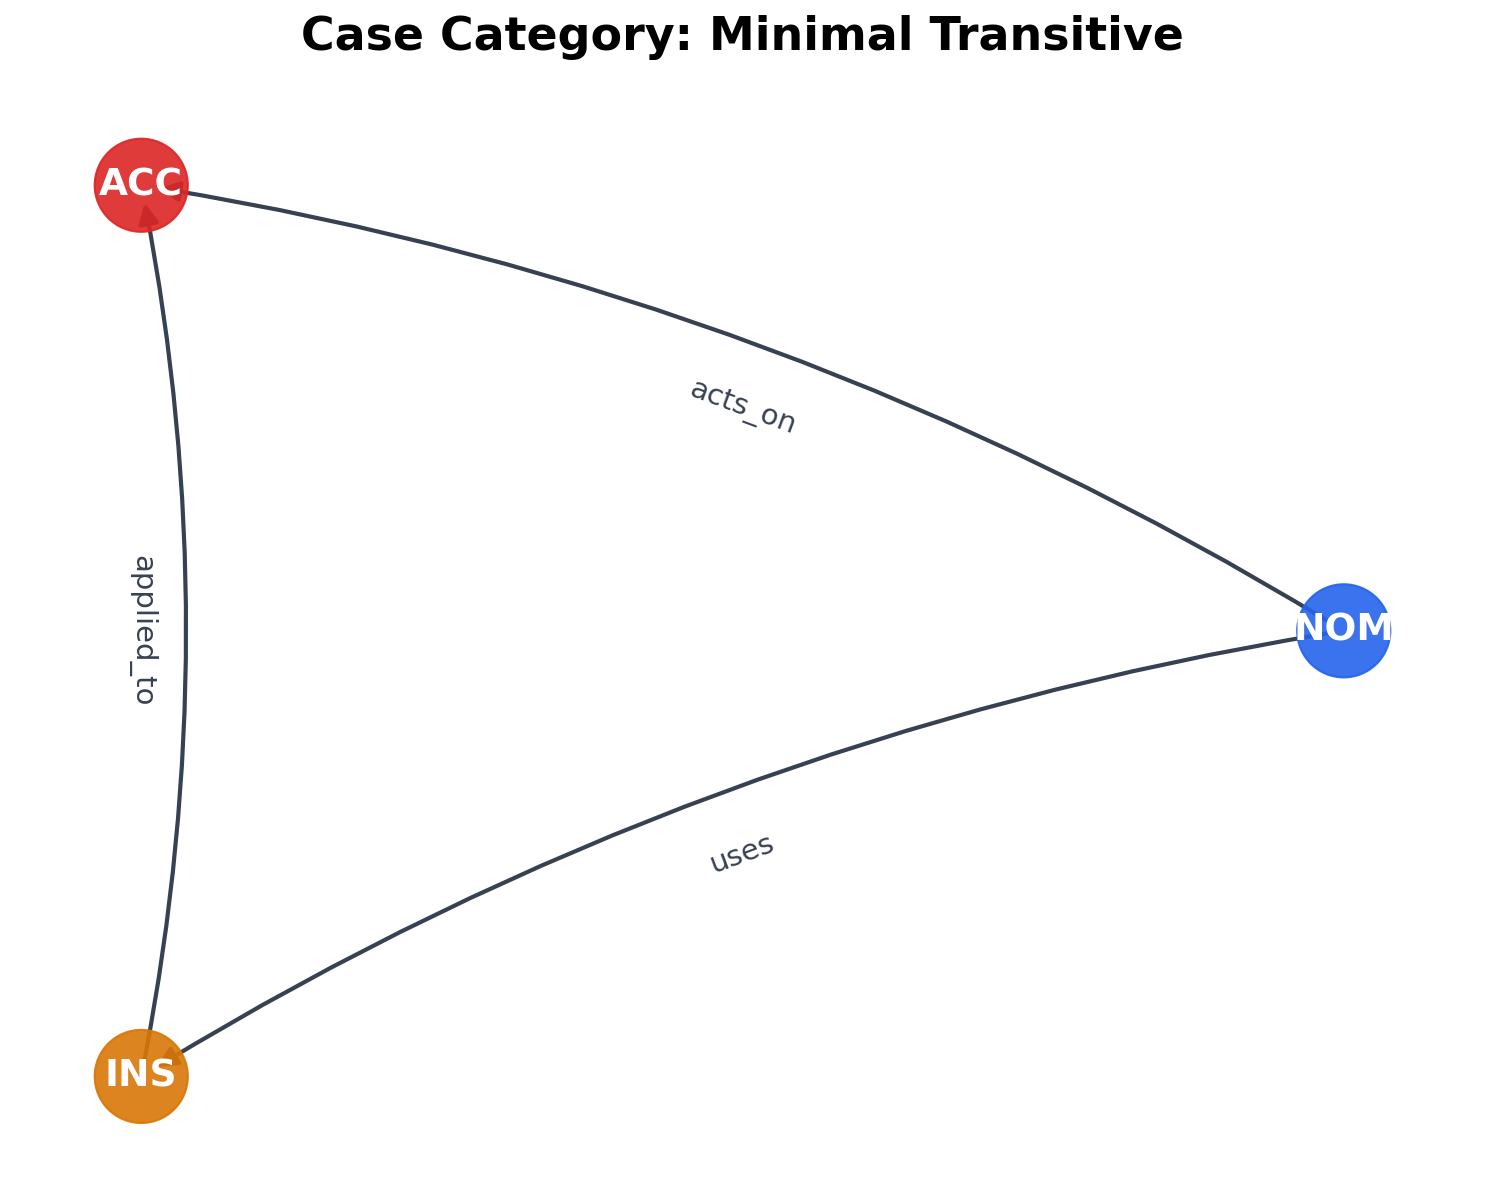
\includegraphics[keepaspectratio,alt={A minimal case category with three objects---Agent (NOM), Patient (ACC), and Instrument (INS)---and three morphisms: `acts\_on' (NOM to ACC), `applied\_to' (INS to ACC), and the composite `acts\_via' (NOM to INS to ACC). The commutative triangle makes the factorization through the instrument role visually immediate, illustrating how two-dimensional layout provides a free-ride inference that linear notation obscures.}]{../figures/case_category_minimal.png}}
\caption{A minimal case category with three objects---Agent (NOM),
Patient (ACC), and Instrument (INS)---and three morphisms: `acts\_on'
(NOM to ACC), `applied\_to' (INS to ACC), and the composite `acts\_via'
(NOM to INS to ACC). The commutative triangle makes the factorization
through the instrument role visually immediate, illustrating how
two-dimensional layout provides a free-ride inference that linear
notation obscures.}\label{fig:case-minimal}
\end{figure}
\end{frame}

\begin{frame}{Five Converging Research Pillars}
\protect\phantomsection\label{five-converging-research-pillars}
The present synthesis draws on five research traditions, each
contributing an essential formal ingredient:

\begin{block}{Pillar 1: Case Systems, Alignment Typology, and
Grammatical Relations}
\protect\phantomsection\label{pillar-1-case-systems-alignment-typology-and-grammatical-relations}
The empirical foundation comes from linguistic typology. We formalize
the case inventory and alignment systems catalogued by Polinsky and
Preminger {[}-@polinsky2015case{]}, Claassen
{[}-@claassen2025alignment{]}, and Wu {[}-@wu2024amis{]} as categories
with case roles as objects and grammatical relations as morphisms.
Dowty's {[}-@dowty1991thematic{]} proto-role theory---which decomposes
thematic roles into clusters of entailments rather than discrete
atoms---motivates our use of enriched (weighted) morphisms.
\end{block}

\begin{block}{Pillar 2: Categorial and Type-Theoretic Grammar}
\protect\phantomsection\label{pillar-2-categorial-and-type-theoretic-grammar}
Lambek's {[}-@lambek1958mathematics{]} syntactic calculus reformulates
grammatical combination as algebraic cancellation in a pregroup,
yielding derivations that can be visualized as Joyal and Street's
{[}-@joyalstreet1991geometry{]} string diagrams. Song
{[}-@song2022act{]} extends this with monadic semantics for root syntax,
showing that category-theoretic structure reaches down to the sublexical
level.
\end{block}

\begin{block}{Pillar 3: Categorical Compositional Distributional
Semantics (DisCoCat)}
\protect\phantomsection\label{pillar-3-categorical-compositional-distributional-semantics-discocat}
The DisCoCat framework {[}@coecke2010mathematical;
@grefenstette2015concrete; @sadrzadeh2013compositional{]} maps pregroup
derivations functorially into vector spaces, enabling empirical
evaluation. Recent extensions include DisCoCirc
{[}@defelice2020discourse; @defelice2022discocirc{]} for discourse-level
coherence and the lambeq library {[}@lorenz2023lambeq{]} for quantum
NLP, which implements the full categorical pipeline on quantum hardware.
\end{block}

\begin{block}{Pillar 4: Enriched Category Theory and Distributional
Measures}
\protect\phantomsection\label{pillar-4-enriched-category-theory-and-distributional-measures}
Fritz et al.'s {[}-@fritz2021enriched{]} enrichment over \([0,1]\)
equips hom-sets with distributional proximity measures. Bradley's
{[}-@bradley2020entropy; -@bradley2024ipam{]} work on topological
operads and categorical magnitude provides information-theoretic
invariants that quantify the ``effective size'' of a linguistic
category---a measure that captures how much distributional information
the category encodes.
\end{block}

\begin{block}{Pillar 5: Topos-Theoretic Bridges and Inter-Theoretic
Transfer}
\protect\phantomsection\label{pillar-5-topos-theoretic-bridges-and-inter-theoretic-transfer}
Caramello's {[}-@caramello2016bridges; -@caramello2021five;
-@caramello2023syntactic{]} bridge technique uses classifying toposes as
transfer points between mathematical theories, enabling results proved
in one formalization of case to port automatically to another. Phillips
{[}-@phillips2024lot{]} strengthens this by showing that the Language of
Thought admits universal constructions in a topos, grounding the
systematicity of case assignment in the deepest structures of
categorical logic.
\end{block}
\end{frame}

\begin{frame}{Unifying Integration: Active Inference and the CEREBRUM
Architecture}
\protect\phantomsection\label{unifying-integration-active-inference-and-the-cerebrum-architecture}
The unifying framework is \textbf{active inference}
{[}@friston2017active{]}, which casts cognition as approximate Bayesian
inference under a generative model. Case-marked commutative diagrams
serve as the structural core of such generative models: each diagram
specifies a pattern of expected relational dependencies, and the agent's
task in understanding (or producing) a sentence is to minimize surprise
relative to this diagrammatic prior. The \textbf{CEREBRUM} architecture
{[}@friedman2024cerebrum{]}---Case-Enabled Reasoning Engine with
Bayesian Representations for Unified Modeling---provides a computational
instantiation of this framework, with case roles as functional
specializations of model components in an active inference cycle.

This integration is not merely metaphorical. The situation semantics of
Barwise and Perry {[}-@barwise1983situations{]} already conceptualized
meaning as structured \emph{situations} with typed constituents---an
ontology that maps naturally onto the objects and morphisms of our case
categories. Active inference adds dynamics: the agent actively samples
evidence to confirm or update its case assignments, using diagrammatic
structure to guide exploration.
\end{frame}

\begin{frame}{Paper Outline and Chapter Overview}
\protect\phantomsection\label{paper-outline-and-chapter-overview}
The remainder of the paper is organized as follows.
\autoref{sec:case-systems} reviews case systems and alignment typology.
\autoref{sec:categorial-grammar} develops the categorial grammar
foundations. \autoref{sec:categorical-semantics} presents DisCoCat and
its extensions. \autoref{sec:enriched-categories} introduces enriched
categories. \autoref{sec:topos-theory} develops the topos-theoretic
bridges. \autoref{sec:cognitive-integration} integrates everything
within active inference and CEREBRUM. \autoref{sec:ai-implications}
develops implications for synthetic and artificial intelligence.
\autoref{sec:conclusion} concludes with future directions.
\end{frame}

\end{document}
